\documentclass[11pt]{article}

\def\chapitre{17}
\def\pagetitle{Structures algébriques.}

\input{/home/theo/MP2I/setup.tex}

\begin{document}

\input{/home/theo/MP2I/title.tex}

\renewcommand*{\s}{\oldstar}

\thispagestyle{fancy}

\section{Loi de composition interne sur un ensemble.}

\subsection{Définitions et propriétés.}

\begin{defi}{\unskip et 2}{}
    On appelle \bf{loi de composition interne} sur un ensemble $E$ (on écrire l.c.i.) une application
    \begin{equation*}
        \s:\begin{cases}
            E \times E &\to \quad E\\
            (x,y) &\mapsto \quad x\s y
        \end{cases}
    \end{equation*}
    On notera que l'image de $(x,y)$ par $\s$ est notée $x\s y$ plutôt que $\s(x,y)$.\\
    Soit $E$ un ensemble et $\s$ une l.c.i. sur $E$.
    \begin{itemize}
        \item La loi $\s$ est dite \bf{associative} si $\forall (x,y,z)\in E^3, ~ (x\s y)\s z = x\s (y \s z)$.
        \item De deux éléments $x$ et $y$ de $E$, on dit qu'ils \bf{commutent} pour $\s$ lorsque $x\s y = y\s x$.
        On dit que la loi $\s$ est \bf{commutative} si $\forall (x,y)\in E^2, ~ x \s y = y \s x$.
        \item On appelle \bf{élément neutre} pour $\s$ tout élément $e\in E$ tel que $\forall x\in E, ~ x \s e = x$ et $e \s x = x$.
    \end{itemize}
\end{defi}

\begin{defi}{Vocabulaire hors-programme.}{}
    Un couple $(E,\s)$, où $E$ est un ensemble et $\s$ une l.c.i. sur $E$ est appelé \bf{magma}.\n
    On dit que ce magma est associatif si $\s$ est associative, commutatif si $\s$ est commutative, et \bf{unifère} s'il existe dans $E$ un élément neutre pour $\s$.
\end{defi}

\begin{prop}{}{}
    Dans un magma unifère, il y a unicité du neutre.
    \tcblower
    Soient $e$ et $e'$ des éléments neutres d'un magma unifère $(E,\s)$.\\
    On a $e\s e' = e = e'$ car $e$ et $e'$ sont neutres pour $\s$ donc $e=e'$.
\end{prop}

\begin{defi}{Partie stable.}{}
    Soit $(E,\s)$ un magma et $A\in\P(E)$. On dit que $A$ est \bf{stable} par $\s$ si
    \begin{equation*}
        \forall (x,y) \in A^2, ~ x \s y \in A.
    \end{equation*}
\end{defi}

\vspace*{-0.1cm}

\begin{defi}{Loi induite.}{}
    Soit $(E,\s)$ un magma et $A\in\P(E)$ stable par $\s$. La restriction de $\s$ à $A^2$:
    \begin{equation*}
        \s : \begin{cases}
            A\times A &\to \quad A\\
            (x,y)&\mapsto\quad x\s y
        \end{cases}
    \end{equation*}
    est une l.c.i. sur $A$ : on l'appelle loi induite par $\s$ sur $A$.
\end{defi}

\vspace*{-0.1cm}

\begin{ex}{Ensembles de nombres.}{}
    \begin{itemize}
        \item $+$ est une l.c.i. associative, commutative avec 0 comme neutre sur $\N,\Z,\Q,\R,\C$.
        \item $\times$ est une l.c.i. associative, commutative, de neutre 1 sur $\N,\Z,\Q,\R,\C$.
        \item $-$ est une l.c.i. non associative, non commutative et sans neutre sur $\Z$. $\N$ n'est pas stable par $-$.
    \end{itemize}
\end{ex}

\vspace*{-0.1cm}

\begin{ex}{Ensemble des parties}{}
    Soit $E$ un ensemble. L'intersection $\cap$ et la réunion $\cup$ définissent des l.c.i. sur $\P(E)$.
    \begin{itemize}
        \item Le magma $(\P(E),\cap)$ est associatif, commutatif et unifère, avec $E$ pour neutre.
        \item Le magma $(\P(E),\cup)$ est associatif, commutatif et unifère, avec $\0$ pour neutre.
    \end{itemize}
\end{ex}

\vspace*{-0.1cm}

\begin{ex}{Ensembles de fonctions et composition.}{}
    Soit $E$ un ensemble. La composition $\circ$ est une l.c.i. sur $E^E$, l'ensemble des fonctions de $E$ vers $E$.\\
    Le magma $(E^E,\circ)$ est associatif et unifère : il admet $\id_E$ pour neutre. Si $|E|\geq2$, il n'est pas commutatif.\\
    L'ensemble des fonctions injectives est stable par $\circ$, de même pour l'ensemble des fonctions surjectives, bijectives.
\end{ex}

\vspace*{-0.1cm}

\begin{defi}{Distributivité d'une loi par rapport à une autre.}{}
    Soit $E$ un ensemble muni de deux l.c.i. $\oplus$ et $\otimes$.\\
    On dit que $\otimes$ est \bf{distributive par rapport à} $\oplus$ si
    \begin{equation*}
        \forall (x,y,z)\in E^3 \quad : \quad \begin{cases}
            x \otimes (y \oplus z) = (x \otimes y) \oplus (x \otimes z)\\
            (y \oplus z) \otimes x = (y \otimes x) \oplus (z \otimes x)
        \end{cases}
    \end{equation*}
    (Si la loi $\oplus$ n'est pas commutative, il est primordial de vérifier les deux égalités.)
\end{defi}

\begin{ex}{}{}
    \begin{itemize}
        \item Dans $\N,\Z,\Q,\R,\C$, la multiplication $\times$ est distributive par rapport à l'addition $+$.
        \item Dans $\P(E)$, $\cap$ est distributive par rapport à $\cup$.
        \item Dans $\P(E)$, $\cup$ est distributive par rapport à $\cap$.
    \end{itemize}
\end{ex}

\subsection{Éléments symétrisables.}

\begin{defi}{Élément symétrisable.}{}
    Soit $(E,\s)$ un magma unifère de neutre $e$, et $x\in E$.\\
    On dit que $x$ est \bf{symétrisable} (ou \bf{inversible}) s'il existe un élément $x'$ dans $E$ tel que
    \begin{equation*}
        x \s x' = e \quad\et\quad x'\s x=e.
    \end{equation*}
\end{defi}

\begin{prop}{Unicité du symétrique / de l'inverse.}{}
    Soit $(E,\s)$ un magma associatif et unifère de neutre $e$.\\
    Si $x$ est un élément de $E$ symétrisable, il existe un unique $x'$ dans $E$ tel que $x\s x'=x'\s x=e$.\\
    On appelle cet élément le \bf{symétrique} de $x$ (ou son inverse), et on le note $x^{-1}$. 
    \tcblower
    Soit $x\in E$ et $x',x''\in E$ tels que :
    \begin{equation*}
        \begin{cases}
            x \s x' = x' \s x = e,\\
            x \s x'' = x'' \s x = e
        \end{cases}
    \end{equation*}
    On a alors $x'\s x \s x'' = (x' \s x)\s x'' = x'' = x'\s(x\s x'') = x'$  donc $x'=x''$.
\end{prop}

\begin{ex}{}{}
    \begin{itemize}
        \item Les inversibles de $(\Z,\times)$ sont $-1$ et $1$.
        \item Les inversibles de $(\R,\times)$ sont les réels non nuls. (admis)
    \end{itemize}
    \tcblower
    On vérifie facilement que $-1$ et $1$ sont inversibles.\\
    Soit $p\in\Z\setminus\{-1,0,1\}$. Supposons par l'absurde qu'il existe $q\in\Z$ tel que $pq=qp=1$.\\
    Alors $|p|\geq2$ et $|q|\geq1$ donc $|p||q|\geq2\cdot 1$ donc $|pq|\geq 2$ donc $1\geq2$, absurde.
\end{ex}

\begin{ex}{}{}
    Les inversibles du magma $(E^E,\circ)$ sont les bijections $f:E\to E$, d'inverse $f^{-1}$.
\end{ex}

\begin{prop}{}{}
    Soit $(E,\s)$ un magma associatif et unifère, et $x,y\in E$.
    \begin{enumerate}
        \item Si $x$ est symétrisable, $x^{-1}$ l'est aussi et $(x^{-1})^{-1}=x$.
        \item Si $x$ et $y$ sont symétrisables, $x\s y$ l'est aussi et
        \begin{equation*}
            (x\s y)^{-1} = y^{-1} \s x^{-1}.
        \end{equation*}
    \end{enumerate}
    \tcblower
    \boxed{1.} Supposons que $x$ est symétrisable, alors $x\s x^{-1}=x^{-1}\s x = e$ : $(x^{-1})^{-1}=x$.\\
    \boxed{2.} Supposons $x$ et $y$ symétrisables. Alors :
    \begin{equation*}
        \begin{cases}
            (x\s y)\s(y^{-1}\s x^{-1}) = x \s (y \s y^{\vspace*{-0.1cm}-1}) \s x^{-1} = x\s x^{-1} = e,\\
            (y^{-1}\s x^{-1})\s(x\s y) = y^{-1}\s(x^{-1}\s x)\s y = y^{-1}\s y = e.
        \end{cases}
    \end{equation*}
    Donc $x\s y$ est inversible, d'inverse $y^{-1}\s x^{-1}$.
\end{prop}

\subsection{Itérés.}

On fixe pour tout ce paragraphe un magma $(E,\s)$ associatif et unifère de neutre $e$.

\begin{defi}{Itérés d'un élément.}{}
    Soit $x\in E$.
    \begin{enumerate}
        \item Pour $n\in \N$, on définit $x^n$ par récurrence sur $n$.
        --- On pose $x^0 = e$.\\
        --- Pour tout $n\in\N$ : $x^{n+1}=x^n\s x$.
        \item Si $x$ est inversible et $n\in\N^*$, on pose $x^{-n}=(x^{-1})^n$.
    \end{enumerate}
\end{defi}

\begin{prop}{Propriétés des itérés.}{}
    \begin{equation*}
        \forall x \in E, ~ \forall (m,n) \in \N^2, ~ x^m \s x^n = x^{m+n} \quad \et \quad (x^m)^n = x^{mn}.
    \end{equation*}
    Si $x$ est inversible, les identités ci-dessus sont vraies pour $(m,n)\in\Z^2$.
    \tcblower
    Soit un élément $x$ de $E$.\n
    Soit $m\in\N$ fixé. Pour $n\in\N$, on note $\P(n):$<< $x^m\s x^n = x^{m+n}$ >>.\\
    \bf{Initialisation.} On a $x^m\s x^0 = x^l \s e = x^{m+0}$.\\
    \bf{Hérédité.} Soit $n\in\N \mid \P(n)$. Alors $x^m\s x^{n+1} = x^m \s x^n \s x = x^{m+n}\s x= x^{m+n+1}$.\\
    \bf{Conclusion.} Par récurrence, $\forall n\in\N, ~ \P(n)$.\n
    Soit $m\in\N$ fixé. Pour $n\in\N$, on note $\m{Q}(n):$<< $(x^m)^n=x^{m\cdot n}$ >>.\\
    \bf{Initialisation.} On a $(x^m)^0=e=x^{m\cdot0}$.\\
    \bf{Hérédité.} Soit $n\in\N\mid\m{Q}(n)$. Alors $(x^m)^{n+1}=(x^m)^n\s x^m = x^{mn}\s x^m = x^{mn+m} = x^{m(n+1)}$.\\
    \bf{Conclusion.} Par récurrence, $\forall n\in\N, ~ \m{Q}(n)$.
\end{prop}

\begin{ex}{Itérés d'éléments qui commutent.}{}
    Soient $x$ et $y$ deux éléments deux $E$ qui commutent. Alors
    \begin{equation*}
        \forall (m,n)\in\N^2, ~ x^m \s y^n = y^n \s x^m \quad\et\quad (x\s y)^n = x^n \s y^n.
    \end{equation*}
    \warning Les identités ci-dessus sont FAUSSES en général lorsque $x$ et $y$ ne commutent pas.
\end{ex}

\subsection{Notations multiplicatives et additives.}

\quad Utiliser la \bf{notation multiplicative}, lorsqu'on travaille avec un magma $(E,\s)$ consiste à ne pas écrire $\s$ lorsqu'on calcule l'image d'un couple $(x,y)\in E^2$. Concrètement, on note alors $xy$ à la place de $x\s y$.\n
\quad Lorsqu'on travaille avec un magma associatif, commutatif et unifère, on pourra utiliser la notation $+$ pour la l.c.i. Le vocabulaire sur les notations introduits plus haut est alors adapté à cette \bf{notation additive}, comme explicité dans le tableau ci-dessous.

\begin{center}
    \begin{tabular}{|c|c|c|c|}
        \hline
        notation l.c.i. & $\s$ & $\cot$ & $+$\\
        \hline
        image de $(x,y)$ & $x\s y$ & $xy$ & $x+y$\\
        \hline
        notation neutre & $e$ & $e$ & 0\\
        \hline
        on dit & symétrisable & inversible & symétrisable\\
        \hline
        on dit & symétrique & inverse & opposé\\
        \hline
        notation symétrique & $x^{-1}$ & $x^{-1}$ & -x\\
        \hline
        notation itéré & $x^n$ & $x^n$ & nx\\
        \hline
    \end{tabular}
\end{center}

\section{Structure de groupe.} 

\subsection{Définition et exemples.}

\begin{defi}{}{}
    On appelle \bf{groupe} un magma associatif et unifère dans lequel tout élément est symétrisable.\n
    Plus précisément, un groupe est la donnée d'un couple $(G,\s)$ où $G$ est un ensemble et $\s$ une l.c.i. tels que
    \begin{enumerate}
        \item $\s$ est associative.
        \item il existe dans $G$ un élément $e$ neute pour $\s$.
        \item tout élément de $G$ est symétrisable.
    \end{enumerate}
    Si de surcroît $\s$ est commutative, on dit que le groupe $(G,\s)$ est \bf{abélien} (ou commutatif).
\end{defi}

\bf{Remarque.} Un groupe n'est jamais vide car il contient au moins son élément neutre.

\begin{prop}{Ensembles de nombres.}{}
    \begin{enumerate}
        \item $(\Z,+)$, $(\Q,+)$, $(\R,+)$ et $(\C,+)$ sont des groupes abéliens.
        \item $(\Q^*, \times)$, $(\R^*, \times)$ et $(\C^*, \times)$ sont des groupes abéliens.
    \end{enumerate}
\end{prop}

\begin{ex}{Ce ne sont pas des groupes.}{}
    \begin{enumerate}
        \item $(\N,+)$ n'est pas un groupe car $1$ n'est pas symétrisable.
        \item $(\Z^*,\times)$ n'est pas un groupe car $2$ n'est pas inversible dans $\Z$.
        \item $(\C,+)$ n'est pas un groupe car $0$ n'a pas d'inverse dans $\C$.
    \end{enumerate}
\end{ex}

\begin{ex}{Vérifier les axiomes de groupe sur une loi artificielle.}{}
    On pose $G=\R^*\times\R$. Pour $(a,b)\in G$ et $(a',b')\in G$ on définit
    \begin{equation*}
        (a,b)\s(a',b')=(aa',ab'+b).
    \end{equation*}
    Montrer que $(G,\s)$ est un groupe.
    \tcblower
    On vérifie chacun des points de la définition de groupe...\\
    $\s$ est-elle une l.c.i. dans $G$ ? $G$ est-il associatif ? Unifère ? Symétrisable ? 
\end{ex}

\begin{defi}{}{}
    Soit $E$ un ensemble non-vide. On appelle \bf{permutation} de $E$ une bijection $\sigma:E\to E$.\\
    On note $S_E$ l'ensemble des permutations de $E$.
\end{defi}

\begin{prop}{$\star$}{}
    $(S_E,\circ)$ est un groupe, appelé \bf{groupe des permutations} de $E$, ou groupe symétrique de $E$.\\
    Dès que $E$ contient au moins 3 éléments, le groupe $S_E$ n'est pas abélien.
    \tcblower
    Soient $\sigma,\sigma'\in S_E$. On a $\sigma\circ\sigma':E\to E$ une bijection comme composée.\\
    --- $\circ$ est une l.c.i. sur $E$.\\
    --- \bf{Associativité.} On sait déjà que $(\F(E,E), \circ)$ est associatif.\\
    --- \bf{Unifère.} $\id_E\in S_E$ est neutre pour $\circ$.\\
    --- \bf{Symétrie.} Si $f\in S_E$, c'est une bijection alors $f^{-1}\in S_E$ et est le symétrique de $f$.\\
    Supposons que $|E|\geq3$. Soient $a,b,c\in E$ différents.\\
    On définit $\sigma$ telle que $\sigma(a)=b$, $\sigma(b)=c$, $\sigma(c)=a$ et $\sigma(x)=x$ pour $x\in E\setminus\{a,b,c\}$.\\
    On définit $\sigma'$ telle que $\sigma'(a)=b$, $\sigma'(b)=a$ et $\sigma'(x)=x$ pour $x\in E\setminus\{a,b\}$.\\
    On a $\sigma'\circ\sigma(a)=a$ et $\sigma\circ\sigma'(a)=c$ donc $\sigma'\circ\sigma\neq\sigma\circ\sigma'$ : pas commutatif.
\end{prop}

\begin{prop}{Produit de deux groupes.}{}
    Soient $(G,\s)$ et $(G',\top)$ deux groupes. On note $e$ le neutre de $G$ et $e'$ celui de $G'$.\\
    Pour $(x,x')$ et $(y,y')$ deux éléments de $G\times G'$, on pose
    \begin{equation*}
        (x,x')\heartsuit(y,y')=(x\s y, x' \top y').
    \end{equation*}
    Muni de la l.c.i. $\heartsuit$, le produit cartésien $G\times G'$ est un groupe, de neutre $(e,e')$.
    \tcblower
    On vérifie chacun des points de la définition de groupe...
\end{prop}

\pagebreak

\begin{prop}{Produit de $n$ groupes.}{}
    Soient $G_1,...,G_n$ $n$ groupes (les l.c.i. étant sous-jacentes et notées multiplicativement).\\
    Pour $(x_1,...,x_n)$ et $(y_1,...,y_n)$ deux éléments $G_1\times ... \times G_n$, on pose
    \begin{equation*}
        (x_1,...,x_n)\heartsuit(y_1,...,y_n)=(x_1y_1,...,x_ny_n).
    \end{equation*}
    Muni de la l.c.i. $\heartsuit$, le produit cartésien $G_1\times ... \times G_n$ est un groupe, de neutre $(e_1,...,e_n)$.
\end{prop}

\subsection{Sous-groupes.}

\begin{defi}{}{}
    Soit $(G,\s)$ un groupe et $H$ une partie de $G$.\\
    On dit que $H$ est un \bf{sous-groupe} de $G$ si $H$ est stable par $\s$ et si $(H,\s)$ est un groupe.
\end{defi}

\begin{prop}{Élément neutre et inverses dans un sous-groupe.}{}
    Soit $(G,\s)$ un groupe et $H$ un sous-groupe de $G$.
    \begin{enumerate}
        \item L'élément neutre du groupe $H$ n'est autre que celui de $G$.
        \item Soit $x\in H$. L'inverse de $x$ dans le groupe $(H,\s)$ et celui dans le groupe $(G,\s)$ sont égaux.
    \end{enumerate}
    \tcblower
    \boxed{1.} Soit $e$ le neutre de $G$. On a $\forall x \in G, ~ e\s x = x\s e = x$ donc $\forall x \in H, ~ e\s x = x\s e = x$ car $H\subset G$.\\
    Par unicité du neutre dans $H$, on a $e$ neutre de $H$.\\
    \boxed{2.} Soit $x\in H$. On note $x'$ l'inverse de $x$ dans $H$ et $x''$ dans $G$.\\
    Alors $x'\s x = x \s x' = e$ et $x''\s x = x\s x'' = e$, donc par unicité du neutre dans $G$, $x'=x''$. 
\end{prop}

\begin{thm}{Caractérisation des sous-groupes.}{}
    Soit $(G,\s)$ un groupe de neutre $e$ et $H\subset G$. On équivalence entre :
    \begin{enumerate}
        \item $H$ est un sous-groupe de $G$.
        \item $
            \begin{cases}
                \bullet ~ e \in H,\\
                \bullet ~ \forall (x,y) \in H^2, ~ x \s y^{-1} \in H
            \end{cases}$
        \item $
            \begin{cases}
                \bullet ~ e \in H\\
                \bullet ~ \forall (x,y) \in H^2, ~ x \s y \in H\\
                \bullet ~ \forall x \in H, ~ x^{-1} \in H
            \end{cases}$
    \end{enumerate}
    \bf{Remarque.} On utilisera presque \bf{toujours} cette caractérisation. 
    \tcblower
    \boxed{\circled{1}\ra\circled{2}} Supposons $H$ sous-groupe de $G$. Alors $H$ est stable par $\s$ et $(H,\s)$ est un groupe.\\
    --- $\bullet$ $e$ est le neutre de $G$, c'est aussi celui de $H$ donc $e\in H$.\\
    --- $\bullet$ Soit $(x,y)\in H^2$. $y^{-1}$ est l'inverse de $y$ et $y^{-1}\in H$, alors $x\s y^{-1}\in H$ par stabilité de $H$ par $\s$.\\
    \boxed{\circled{2}\ra\circled{3}} Supposons $e\in H$ et $\forall (x,y) \in H^2, ~ x \s y^{-1} \in H$.\\
    --- $\bullet$ $e\in H$ donc $e\in H$.\\
    --- $\bullet$ Soient $(x,y)\in H^2$ : $x\s y= x\s(y^{-1})^{-1}\in H$ par hypothèse.\\
    --- $\bullet$ Soit $x\in H$, on a $x^{-1}=e\s x^{-1}\in H$ car $e,x\in H$.\\
    \boxed{\circled{3}\ra\circled{1}} Supposons $e\in H$, $\forall (x,y)\in H^2, ~ x\s y\in H$ et $\forall x \in H, ~ x^{-1} \in H$.\\
    --- $\bullet$ $H$ est stable par $\s$ car $\forall (x,y)\in H^2, ~ x\s y\in H$ et $\s$ est l.c.i. sur $H$ par déf.\\
    --- $\bullet$ $\s$ est associative sur $H$ car elle l'est sur $G$.\\
    --- $\bullet$ $H$ est unifère car $e$ est neutre et $e\in H$.\\
    --- $\bullet$ tout élément de $H$ est symétrisable car $\forall x \in H, ~ x^{-1} \in H$.
\end{thm}

\begin{prop}{Sous-groupes usuels.}{}
    \begin{enumerate}
        \item $(\Q,+)$ est un sous-groupe de $(\R,+)$, qui est lui-même un sous-groupe de $(\C,+)$.
        \item $\R_+^*$ est un sous-groupe de $(\R^*,\times)$.
        \item $\mathbb{U}$ et $\mathbb{U}_n$ sont des sous-groupes de $(\C^*, \times)$.
    \end{enumerate}
\end{prop}

\begin{ex}{Une intersection de sous-groupes est un sous-groupe. $\star$}{}
    Soient $H$ et $H'$ deux sous-groupes d'un groupe $(G,\s)$. Montrer que $H\cap H'$ est sous-groupe de $G$.
    \tcblower
    $\bullet$ Soit $e$ le neutre de $G$, on a alors $e\in H$ et $e\in H'$ car sous-groupes donc $e\in H\cap H'$.\\
    $\bullet$ Soient $x,y\in H\cap H'$.\\
    --- On a $x\in H$ et $y\in H$ donc $x\s y^{-1}\in H$ car $H$ est un groupe.\\
    --- On a $x\in H'$ et $y\in H'$ donc $x\s y^{-1}\in H'$ car $H'$ est un groupe.\\
    --- Alors $x\s y^{-1}\in H\cap H'$.
\end{ex}

\pagebreak

\begin{ex}{Une union de sous-groupes n'est pas toujours un sous-groupe.}{}
    Montrer que $\mathbb{U}_2\cup\mathbb{U}_3$ n'est pas un sous-groupe de $(\C^*,\times)$.\n
    On note $\ds H=\bigcup_{n\in\N^*}\mathbb{U}_n$. Montrer que $H$ est un sous-groupe de $(\C^*,\times)$.
    \tcblower
    \boxed{1.} On a $\mathbb{U}_2\cup \mathbb{U}_3=\{-1,1,j,j^2\}$ et $-1\times j = -j \notin \mathbb{U}_2\cup\mathbb{U}_3$ : pas stable par $\times$.\\
    \boxed{2.} On a $1\in H$ car $1\in \mathbb{U}_1$.\\
    $\bullet$ Soient $z,\tilde{z}\in H$ : $\exists k,\tilde{k}\in N^* \mid z \in \mathbb{U}_k \et \tilde{z}\in\mathbb{U}_{\tilde{k}}$ donc $(z\cdot\tilde{z})^{k\tilde{k}}=(z^{k})^{\tilde{k}}(\tilde{z}^{\tilde{k}})^k=1$ donc $z\tilde{z}\in\mathbb{U}_{k\tilde{k}}\subset H$.\\
    $\bullet$ Soit $z\in H$ : $\exists p \in \N^* \mid z \in \mathbb{U}_p$, or $\mathbb{U}_p$ est un groupe donc $z^{-1}\in\mathbb{U}_p\subset H$.
\end{ex}

\begin{ex}{Centre d'un groupe. $\star$}{}
    Soit $(G,\s)$ un groupe. On note
    \begin{equation*}
        Z(G)=\{x\in G \mid \forall a \in G, ~ x \s a = a \s x\}.
    \end{equation*}
    Montrer que $Z(G)$ est un sous-groupe de $G$.
    \tcblower
    $\bullet$ Soit $e$ le neutre de $G$. On a $\forall a \in G, ~ e \s a = a \s e = a$ donc $e\in Z(G)$.\\
    $\bullet$ Soient $a,b\in Z(G)$ et $x\in G$. On a $(a\s b)\s x = a \s x \s b = x \s (a \s b)$ donc $a\s b \in Z(G)$.\\
    $\bullet$ Soient $x\in Z(G)$ et $a\in G$. On a $x^{-1}\s a = (a^{-1} \s x)^{-1} = ( x \s a^{-1})^{-1} = a \s x^{-1}$ donc $x^{-1}\in Z(G)$.\\
    Par caractérisation, le centre d'un groupe est un sous-groupe.
\end{ex}

\begin{prop}{Sous-groupes de $(\Z,+)$ (programme de spé). $\star\star$}{}
    Pour $n\in\N$, on note $n\Z=\{nk\mid k \in \Z\}$.\\
    Les sous-groupes de $(\Z,+)$ sont exactement les $n\Z$, avec $n\in\N$.
    \tcblower
    Soit $n\in\N$. Montrons que $n\Z$ est un sous-groupe de $\Z$ :\\
    --- $\bullet$ $0\in n\Z$ car $0 = n0$.\\
    --- $\bullet$ Soient $p,p'\in n\Z$ : $\exists k,k' \in \Z \mid p=kn \et p'=k'n$, alors $p+p'=(k+k')n \in n\Z$.\\
    --- $\bullet$ Soit $p\in\Z$ : $\exists k \in \Z \mid p = kn$ donc $p^{-1}=-p=(-k)n\in n\Z$.\\
    Par caractérisation, c'est bien un sous-groupe de $\Z$.\n
    Soit $H$ un sous-groupe de $\Z$. Montrons qu'il existe $n\in\N$ tel que $H=n\Z$.\\
    $\to$ Cas particulier : $H=\{0\}$, alors $H=0\Z$. Supposons $H\neq\{0\}$ pour la suite.\\
    On a alors $H\cap\N^*$ une partie non-vide de $\N^*$. Notons $n$ son plus petit élément. Montrons que $H=n\Z$.\\
    \boxed{\supset} Soit $p\in n\Z$ : $\exists k \in \Z \mid p = nk$ : $p$ est itéré de $n$ avec $n\in H$ donc $p\in H$.\\
    \boxed{\subset} Soit $p\in H$ : $\exists!(q,r)\in\Z^2 \mid p = nq+r \et 0 \leq r < n$ (division euclidienne).\\
    --- Alors $r=p-nq$ avec $p\in H \et nq\in H$ donc $r\in H$.\\
    --- Supposons $r\neq0$, alors $r\in H\cap \N^*$, or $n=\min(H\cap\N^*)$ et $r<n$ : absurde !\\
    --- Donc $r=0$ et $p=nq$ donc $p\in n\Z$.\n
    Par double-inclusion, $H=n\Z$.
\end{prop}

\begin{ex}{(*) Sous-groupes de $(\R,+)$.}{}
    Pour $a\in\R_+$, on note $a\Z=\{ak\mid k\in \Z\}$.\\
    Soit $H$ un sous-groupe de $(\R,+)$. Ou bien il existe $a\in\R_+$ tel que $H=a\Z$, ou bien $H$ est dense dans $\R$.
\end{ex}

\subsection{Morphismes de groupes.}

\begin{defi}{}{}
    Soient $(G,\s)$ et $(G',\top)$ deux groupes.\n
    On appelle \bf{morphisme de groupe} de $G$ dans $G'$ toute application $f:G\to G'$ telle que
    \begin{equation*}
        \forall (x,y)\in G^2, ~ f(x \s y) = f(x) \top f(y).
    \end{equation*}
    Si de surcroît $f$ est bijective, on dit qu'une telle application $f$ est un \bf{isomorphisme} de groupes.\\
    Un morphisme d'un groupe $G$ vers lui même est appelé \bf{endomorphisme} de $G$.\\
    Si un tel endomorphisme est bijectif, on parle d'\bf{automorphisme} de $G$.
\end{defi}

\begin{defi}{}{}
    On dit que deux groupes sont \bf{isomorphes} s'il existe un isomorphisme de l'un vers l'autre.
\end{defi}

\begin{ex}{}{}
    \begin{itemize}
        \item L'exponentielle réelle est un isomorphisme de $(\R,+)$ dans $(\R^*,\times)$.
        \item L'exponentielle complexe est un morphisme de groupes de $(\C,+)$ dans $(\C^*,\times)$.
        \item $t\mapsto e^{it}$ est un morphisme de groupes de $(\R,+)$ dans $(\mathbb{U},\times)$.
        \item Le logarithme népérien est un isomorphisme de groupes de $(\R^*,\times)$ dans $(\R,+)$.
    \end{itemize}
\end{ex}

\begin{ex}{}{}
    Justifier que les groupes $(\R^2,+)$ et $(\C,+)$ sont isomorphes.
    \tcblower
    On pose $f:(a,b)\mapsto a+ib$. Soient $(a,b)$ et $(a',b')$ dans $\R^2$.
    \begin{align*}
        f((a,b) + (a',b')) &= f((a+a',b+b')) = (a+a') + i(b+b') = a+ib + a'+ib' \\&= f(a,b) + f(a',b').
    \end{align*}
    La fonction $f$ est un morphisme de groupes de $(\R^2,+)$ dans $(\C,+)$.\n
    Elle est bijective par unicité de la forme algébrique : c'est un isomorphisme. Les groupes sont donc isomorphes.
\end{ex}

\begin{prop}{$\star$}{}
    Soient $G$ et $G'$ deux groupes de neutres respectifs $e$ et $e'$, et $f:G\to G'$ un morphisme de groupes.
    \begin{enumerate}
        \item $f(e)=e'$.
        \item $\forall x \in G, ~ f(x^{-1}) = f(x)^{-1}$.
        \item $\forall x \in G, ~ \forall p\in\Z, ~ f(x^p) = f(x)^p$.
        \item Si $H$ est un sous-groupe de $G$, alors $f(H)$ est un sous-groupe de $G'$.
        \item Si $H'$ est un sous-groupe de $G'$, alors $f^{-1}(H')$ est un sous-groupe de $G$.
        \item Si $f$ est un isomorphisme de $G$ vers $G'$, alors $f^{-1}$ est un isomorphisme de $G'$ vers $G$.
    \end{enumerate}
    \tcblower
    \boxed{1.} On a $f(e)=f(e\cdot e)=f(e)\cdot f(e) = f(e)^{-1}\cdot f(e)\cdot f(e)=f(e)^{-1}\cdot f(e)=e'$.\\
    \boxed{2.} Soit $x\in G$. On a $f(x\cdot x^{-1})=f(x)f(x^{-1})=f(e)=e'$ donc par unicité de l'inverse $f(x)^{-1}=f(x^{-1})$.\\
    \boxed{3.} Soit $x\in G$. Par récurrence sur $p\in\N$.\\
    --- \bf{Initialisation.} $f(x^0)=f(e)=e'=f(x)^0$.\\
    --- \bf{Hérédité.} Soit $p\in\N\mid f(x^p)=f(x)^p$. Alors $f(x^{p+1})=f(x^p\cdot x)=f(x)^pf(x)=f(x)^{p+1}$.\\
    \boxed{4.\star} Soit $H$ un sous-groupe de $G$.\\
    --- $\bullet$ $e'\in f(H)$ car $e\in H$.\\
    --- $\bullet$ Soient $y,\tilde{y}\in f(H)$, d'antécédents $x,\tilde{x}$ : $y\tilde{y}^{-1}=f(x)f(\tilde{x})^{-1}=f(x\cdot\tilde{x}^{-1})\in f(H)$.\\
    Par caractérisation, $f(H)$ est un sous-groupe de $G'$.\\
    \boxed{5.\star} Soit $H'$ un sous-groupe de $G'$.\\
    --- $\bullet$ $e\in f^{-1}(H)$ car $e'\in H'$.\\
    --- $\bullet$ Soient $x,\tilde{x}\in f^{-1}(H)$ : $f(x\tilde x^{-1})=f(x)f(\tilde{x})^{-1}\in H$ par stabilité puisque $f(x)$ et $f(\tilde{x})^{-1}$ dans $H$.\\
    Par caractérisation, $f^{-1}(H')$ est un sous-groupe de $G$.\\
    \boxed{6.} Soit $f$ un isomorphisme de $G$ vers $G'$. Sa réciproque $f^{-1}$ existe.\\
    --- Soient $y,y'\in G'$ : $f^{-1}(yy')=f^{-1}(f(f^{-1}(y)))f(f^{-1}(f(y')))=f^{-1}(f(f^{-1}(y)f^{-1}(y')))=f^{-1}(y)f^{-1}(y')$.
\end{prop}

\begin{defi}{}{}
    Soient $G$ et $G'$ deux groupes de neutres respectifs $e$ et $e'$, et $f:G\to G'$ un morphisme de groupes.
    \begin{enumerate}
        \item On appelle \bf{noyau} de $f$ et on note $\Ker f$ l'ensemble
        \begin{equation*}
            \Ker f = \{x \in G \mid f(x)=e'\}.
        \end{equation*}
        \item On appelle \bf{image} de $f$ et on note $\Im f$ l'ensemble
        \begin{equation*}
            \Im f = \{y \in G' \mid \exists x \in G ~:~ y = f(x)\}.
        \end{equation*}
    \end{enumerate}
\end{defi}

\begin{prop}{$\star\star$}{}
    Soient $G$ et $G'$ deux groupes de neutres respectifs $e$ et $e'$, et $f:G\to G'$ un morphisme de groupes.
    \begin{enumerate}
        \item $\Ker f$ est un sous-groupe de $G$ et
        \begin{center}
            $f$ est injective $\iff$ $\Ker f = \{e\}$.
        \end{center} 
        \item $\Im f$ est un sous-groupe de $G'$ et
        \begin{center}
            $f$ est surjective $\iff$ $\Im f = G'$.
        \end{center}
    \end{enumerate}
    \tcblower
    \boxed{1.} On a $\Ker f=f^{-1}(\{e'\})$ donc $\Ker f$ est un sous-groupe de $G$ comme image réciproque du sous-groupe $\{e'\}$.\\
    \boxed{\ra} Supposons $f$ injective.\\
    --- $\bullet$ $e\in\Ker f$ car $\Ker f$ est un sous-groupe de $G$.\\
    --- $\bullet$ Soit $x\in\Ker f$. Alors $f(x)=f(e)=e'$ et par injectivité de $f$, $x=e$.\\
    Par double inclusion, $\Ker f = \{e\}$.\\
    \boxed{\la} Supposons $\Ker f = \{e\}$. Soient $x,x'\in G$ tels que $f(x)=f(x')$.\\
    On a $f(x)f(x)^{-1}=f(x')f(x)^{-1}$ donc $e'=f(x')f(x)^{-1}=f(x'x^{-1})$.\\
    Alors $x'x^{-1}\in\Ker f$ : $x'x^{-1}=e$, on multiplie par $x$ à droite : $x'=x$.\n
    \boxed{2.} $\Im f = f(G)$ est l'image d'un sous-groupe de $G$ par un morphisme, c'est un sous-groupe de $G'$.\\
    On a déjà l'équivalence, vraie pour n'importe quelle application de $\F(G,G')$.
\end{prop}

\section{Structure d'anneau.}

\subsection{Définitions et règles de calcul.}

\begin{defi}{}{}
    On appelle \bf{anneau} tout triplet $(A,+,\times)$, où $A$ est un ensemble et $+$ et $\times$ des l.c.i telles que
    \begin{itemize}
        \item $(A,+)$ est un groupe abélien, de neutre $0_A$.
        \item $(A,\times)$ est un magma associatif et unifère, de neutre $1_A$.
        \item $\times$ est distributive par rapport à $+$.
    \end{itemize}
    Les lois $+$ et $\times$ sont appelées respectivement \bf{addition} et \bf{multiplication} de l'anneau $A$.\\
    Si de surcroît $\times$ est commutative, on dit que l'anneau $A$ est commutatif.
\end{defi}

\begin{ex}{Ensembles de nombres.}{}
    $(\Z,+,\times)$, $(\Q,+,\times)$, $(\R,+,\times)$ et $(\C,+,\times)$ sont des anneaux commutatifs.
\end{ex}

\begin{ex}{Anneau de fonctions.}{}
    On rappelle que, pour $X$ une partie de $\R$, $\F(X,\R)$, ensemble des fonctions définies sur $X$ et à valeurs réelles a été muni d'une addition et d'une multiplication de la manière suivante :
    \begin{equation*}
        \forall f,g\in\F(X,R), \quad f+g=\begin{cases}
            X&\to\quad \R\\x&\mapsto\quad f(x)+g(x)
        \end{cases} ~\et~ f\times g : \begin{cases}
            X &\to \R\\
            x &\mapsto \quad f(x)g(x)
        \end{cases}
    \end{equation*}
    Le triplet $(\F(X,\R), +, \times)$ est un anneau commutatif.\\
    L'élément neutre pour $+$ est la fonction nulle sur $X$.\\
    L'élément neutre pour $\times$ est la fonction constante sur $X$ égale à $1$.\\
    En particulier, $(\R^\N,+,\times)$ est un anneau commutatif : celui des suites.
\end{ex}

\begin{ex}{Pas des anneaux.}{}
    \begin{itemize}
        \item $(2\Z,+,\times)$ n'est pas un anneau car il n'y a pas de neutre pour $\times$.
        \item $(\F(\R,\R),+,\circ)$ n'est pas un anneau car $\circ$ n'est pas distributive par rapport à $+$.
    \end{itemize}
\end{ex}

\begin{prop}{}{}
    Soit $(A,+,\times)$ un anneau. En utilisant la notation multiplicative pour la loi $\times$,
    \begin{enumerate}
        \item $\forall a \in A, ~ 0_A\times a = a \times 0_A = 0_A$.
        \item $\forall (a,b)\in A^2, ~ a(-b)=(-a)b=-(ab)$.
        \item $\forall (a,b)\in A^2, ~ (-a)(-b)=ab$.
        \item $\forall (a,b)\in A^2, ~ \forall n \in \Z, ~ a(nb)=(na)b=n(ab)$.
    \end{enumerate}
\end{prop}

\begin{prop}{Identités remarquables : si ça commute, d'accord.}{}
    Soit $(A,+,\times)$ un anneau et $(a,b)\in A^2$.
    \begin{enumerate}
        \item Si $ab=ba$, alors $\ds\forall n \in \N, ~ (a+b)^n=\sum_{k=0}^n\binom{n}{k}a^kb^{n-k}$.
        \item Si $ab=ba$, alors $\ds\forall n \in \N^*, ~ a^n-b^n=(a-b)\sum_{k=0}^{n-1}a^kb^{n-k-1}$.
    \end{enumerate}
    \tcblower
    Exactement les mêmes preuves que lorsqu'on $A=\R$.
\end{prop}

\subsection{Groupe des inversibles dans un anneau.}

\begin{defi}{}{}
    Dans un anneau $(A,+,\times)$, les \bf{inversibles} sont les éléments de $A$ inversibles pour la loi $\times$.\\
    L'ensemble des éléments de $A$ qui sont inversibles sera noté $U(A)$.
\end{defi}

\begin{ex}{}{}
    \begin{itemize}
        \item $U(\Z)=\{-1,1\}$.
        \item $U(\R)=\R^*$.
        \item Pour $X\subset\R$, $U(\F(X,\R))$ est l'ensemble des fonctions ne s'annulant pas sur $X$.
    \end{itemize}
\end{ex}

\begin{prop}{}{}
    Si $(A,+,\times)$ est un anneau, $(U(A),\times)$ est un groupe. On l'appelle \bf{groupe des inversibles}.\\
    On a notamment
    \begin{equation*}
        \forall (a,b)\in(U(A))^2, ~ ab\in U(A) \quad\et\quad (ab)^{1}=b^{-1}a^{-1}.
    \end{equation*}
\end{prop}

\subsection{Nilpotents dans un anneau.}

\begin{defi}{}{}
    Dans un anneau $(A,+,\times)$, on dit d'un élément $a\in A$ qu'il est \bf{nilpotent} s'il possède une puissance nulle, c'est à dire :
    \begin{equation*}
        \exists p \in \N^* \mid a^p=0_A.
    \end{equation*}
\end{defi}

\begin{ex}{}{}
    Soit $(A,+,\times)$ un anneau et $(a,b)\in A^2$.
    \begin{enumerate}
        \item Montrer que si $a$ est nilpotent, et si $b$ commute avec $a$, alors $ab$ est nilpotent.
        \item Montrer que si $ab$ est nilpotent, alors $ba$ est nilpotent. 
    \end{enumerate}
    \tcblower
    \boxed{1.} Soit $a$ nilpotent : $\exists p \in \N^* \mid a^p = 0_A$. Alors $(ab)^p=a^pb^p=0_Ab^p=0_A$.\\
    \boxed{2.} Soient $a,b\in A$ tel que $\exists p \in \N^* \mid (ab)^p = 0_A$. Alors $(ba)^{p+1}=b(ab)^pa=b0_Aa=0_A$?
\end{ex}

\begin{ex}{}{}
    Soit $(A,+,\times)$ un anneau non réduit à $\{0_A\}$ et $a\in A$ nilpotent d'ordre $p$.
    \begin{enumerate}
        \item Montrer que $a$ n'est pas inversible.
        \item Montrer que $1_A-a$ est inversible et exprimer son inverse.
    \end{enumerate}
    \tcblower
    \boxed{1.} Supposons $a$ inversible. Alors $a^p$ l'est aussi, $1_A=a^{-p}a^p=a^{-p}0_A=0_A$, absurde.\\
    \boxed{2.} $\ds\left( 1_A-a \right)\sum_{k=0}^{p-1}a^k=1_A-a^p=1_A$, de même a droite.
\end{ex}

\subsection{Sous-anneaux, morphismes d'anneaux.}

\begin{prop}{}{}
    Soit $(A,+,\times)$ un anneau et $B\subset A$. On dit que $B$ est un \bf{sous-anneau} de $A$ si
    \begin{itemize}
        \item $\forall (a,b)\in B^2, ~ a-b\in B$.
        \item $\forall (a,b)\in B^2, ~ ab \in B$.
        \item $1_A\in B$.
    \end{itemize}
    Muni des lois induites par $+$ et $\times$, $B$ est un anneau.
    \tcblower
    Montrons que $(B,+)$ est un groupe abélien.\\
    --- $\bullet$ $1_A\in B$ donc $1_A-1_A\in B$ donc $0_A\in B$.\\
    --- $\bullet$ $\forall (a,b)\in B, ~ a-b \in B$.\\
    Par caractérisation c'est un sous groupe, abélien car $(A,+)$ l'est.\\
    Montrons que $(B,\times)$ est un magma unifère et associatif.\\
    --- $\bullet$ $B$ est stable par $\times$.\\
    --- $\bullet$ Associatif car $\times$ l'est dans $A$.\\
    --- $\bullet$ Unifère car $1_A\in B$ et est neutre pour $\times$.\\
    $\times$ se distribue déjà sur $+$ dans $A$, donc aussi dans $B$.
\end{prop}

\begin{ex}{}{}
    \begin{itemize}
        \item $A$ est un sous-anneau de $A$. Si $0_A\neq1_A$, alors $\{0_A\}$ n'est pas un sous-anneau de $A$.
        \item Montrer que $\Z$ est le seul sous-anneau de $\Z$.
    \end{itemize}
\end{ex}

\begin{ex}{Anneau de Gauss. $\star$}{}
    Soit l'ensemble
    \begin{equation*}
        \Z[i]=\{a+ib \mid (a,b) \in \Z^2\}.
    \end{equation*}
    Montrer que $(\Z[i], +, \times)$ est un anneau commutatif et déterminer ses éléments inversibles.
    \tcblower
    Vérifions qu'il s'agit d'un sous-anneau de $(\C,+,\times)$.\\
    Soit $(z,z')\in\Z[i]$ : $\exists! (a,b)\in\Z^2\mid z=a+ib$ et $\exists!(a',b')\in\Z^2\mid z'=a'+ib'$.\\
    --- $\bullet$ $1=1+0i$ et $(1,0)\in\Z^2$ donc $1\in\Z[i]$.\\
    --- $\bullet$ On a $z-z'=(a-a')+i(b-b')$ donc $z-z'\in\Z[i]$.\\
    --- $\bullet$ On a $zz'=(aa'-bb')+i(ab'+a'b)$ donc $zz'\in\Z[i]$.\\
    Donc c'est bien un anneau.\n
    Soit un inversible $z=a+ib$ de $\Z[i]$. On a $zz'=1$ donc $|zz'|=1$ donc $|z||z'|=1$.\\
    On a que $|z|$ et $|z'|$ sont entiers donc $|z|=|z'|=1$, donc $z\in\{\pm1,\pm i\}$.\\
    On vérifie facilement que c'est exactement l'ensemble des inversibles de $\Z[i]$.
\end{ex}

\pagebreak

\begin{defi}{}{}
    Soient $(A,+,\times)$ et $(A',+,\times)$ deux anneaux.\\
    On appelle \bf{morphisme d'anneaux} de $A$ dans $A'$ toute application $f:A\to A'$ telle que
    \begin{itemize}
        \item $\forall (a,b)\in A^2, ~ f(a+b)=f(a)+f(b)$,
        \item $\forall (a,b)\in A^2, ~ f(ab)=f(a)r(b)$,
        \item $f(1_A)=1_{A'}$.
    \end{itemize}
    Si de surcroît $f$ est bijective, on dit qu'une telle application $f$ est un \bf{isomorphisme} d'anneaux.
\end{defi}

\begin{ex}{}{}
    La conjugaison
    \begin{equation*}
        \nt{conj}:\begin{cases}
            \C &\to \quad \C\\
            z &\mapsto \quad \ov{z}
        \end{cases}
    \end{equation*}
    est un isomorphisme de l'anneau $(\C,+,\times)$ dans lui-même.
\end{ex}

\subsection{Anneaux intègres.}

\begin{defi}{}{}
    Soit $(A,+,\times)$ un anneau. On dit d'un élément $a$ de $A$ qu'il est un \bf{diviseur de zéro} si $a\neq 0_A$ et s'il existe un élément $b$ dans $A\setminus\{0_A\}$ tel que $ab=ba=0_A$.
\end{defi}

\begin{ex}{}{}
    \begin{itemize}
        \item Dans l'anneau $(\Z,+,\times)$, il n'y a pas de diviseurs de zéro.
        \item Dans l'anneau $(\R^\R,+,\times)$, il existe des diviseurs de zéro.
    \end{itemize}
\end{ex}

\begin{defi}{}{}
    On appelle anneau \bf{intègre} tout anneau commutatif sans diviseurs de zéro. Dans un tel anneau,
    \begin{equation*}
        \forall (a,b)\in A^2 \quad (ab=0_A) \ra (a = 0_A ~\ou~ b=0_A).
    \end{equation*}
\end{defi}

\begin{ex}{}{}
    $\Z$ est un anneau intègre, l'anneau $\K[X]$ des polynômes aussi, mais pas celui des matrices $M_n(\K)$ ($n\geq2$).
\end{ex}

\section{Structure de corps.}

\subsection{Définitions et exemples.}

\begin{defi}{}{}
    On appelle \bf{corps} tout anneau commutatif $(K,+,\times)$ non réduit à $\{0_K\}$ dans lequel tout élément non nul est inversible.
\end{defi}

\begin{prop}{}{}
    Tout corps est un anneau intègre, la réciproque est fausse.
    \tcblower
    Soit $(K,+,\times)$ un corps. C'est un anneau commutatif.\\
    Supposons qu'il existe un diviseur de zéro, noté $x\in K$.\\
    Alors $x\neq0_K$  et $\exists y \in K\setminus\{0_K\} \mid xy=0_K$ et $yy^{-1}=1_K$ donc $y^{-1}xy=y^{-1}0_K$ donc $x=0_K$. Absurde.
\end{prop}

\begin{ex}{$\star$}{}
    Soit
    \begin{equation*}
        \Q[\sqrt{2}]=\left\{x\in\R \mid \exists (a,b)\in\Q^2, ~ x = a+b\sqrt{2}\right\}.
    \end{equation*}
    Montrer que $\Q[\sqrt{2}]$ est un corps.
    \tcblower
    --- $\bullet$ $\Q[\sqrt{2}]$ est un sous-anneau de $(\R,+,\times)$.\\
    --- $\bullet$ $\Q[\sqrt{2}]$ est commutatif car $\R$ l'est.\\
    Soit $x\in\Q[\sqrt{2}]$ non nul, $\exists (a,b)\in\Q^2\mid x=a+b\sqrt{2}$.\\
    Alors $(a+b\sqrt{2})(a-b\sqrt{2})=a^2-2b^2$ donc $(a+b\sqrt{2})\times\left( \frac{a}{a^2-2b^2} + \frac{b}{a^2-2b^2} \right)=1$.\\
    Notons $c=\frac{a}{a^2-2b^2}$ et $d=\frac{b}{a^2-2b^2}$. On a $c+d\sqrt{2}$ inverse de $a+b\sqrt{2}$. Montrons que $a^2-2b^2\neq0$.\\
    Supposons que $a^2-2b^2=0$, alors $a^2=2b^2$ et si $b=0$, alors $a=0$, impossible.\\
    Si $b\neq0$, alors $\frac{a^2}{b^2}=2$ donc $\left|\frac{a}{b}\right|=\sqrt{2}$, absurde car $\sqrt{2}\notin\Q$.\\
    Alors $\Q[\sqrt{2}]$ est un corps.
\end{ex}

\subsection{Notation fractionnaire dans un corps.}

Soit $(K,+,\times)$ un corps, $a\in K$ et $b\in K^*$. On note $ab^{-1}=\frac{a}{b}$.\\
Pour $(a,c)\in K^2$ et $(b,d)\in(K^*)^2$, on peut vérifier que
\begin{equation*}
    \frac{a}{b}+\frac{c}{d}=\frac{ad+bc}{bd} \qquad \frac{a}{b}\times\frac{c}{d}=\frac{ac}{bd} \qquad \frac{a}{b}=\frac{c}{d}\iff ad = bc \qquad \frac{1}{a}=a^{-1}.
\end{equation*}

\subsection{Corps des fractions d'un anneau intègre.}

\begin{thm}{}{}
    Pour tout anneau intègre $A$, il existe un unique corps commutatif $K$ contenant $A$ et vérifiant
    \begin{equation*}
        \forall x \in K, ~ \exists (a,b) \in A\times A^* \mid x = \frac{a}{b}. 
    \end{equation*}
    Le corps $K$ est appelé \bf{corps des fractions} de l'anneau $A$.
\end{thm}

\bf{Exemple.} Le corps des fractions de $\Z$ n'est autre que $\Q$.

\section{Exercices.}

\subsection*{Groupes, sous-groupes, morphismes de groupes.}

\begin{exercice}{$\bbw$}{}
    Soit $(E,\s)$ un magma associatif fini.\\
    Démontrer qu'il existe dans $E$ un élément idempotent, c'est-à-dire un élément $x$ tel que $x^2=x$.
    \tcblower
    Soit $x\in E$. On considère la suite $(u_n)$ telle que $u_0=1$ et $\forall n \in \N, ~ u_{n+1}=u_n^2$. Soit $n\in\N$.\\
    Puisque $E$ est fini, $\exists p>q \in \N \mid u_{2p}=u_{2q}$ donc $x^{2p}=x^{2q}$.\\
    Alors on pose $n=p-q$ et $a=x^{2p}$. Ainsi : $a^{2^n}=a$.\\
    Si $n=1$, $a$ est idempotent. Sinon, on a:
    \begin{equation*}
        a^{2^{n}-1}a^{2^{n}-1}=a^{2^{n+1}-2}=a^{2^n}a^{2^n-2}=aa^{2^n-2}=a^{2^n-1}
    \end{equation*}
    Donc $a^{2^n-1}$ est idempotent.
\end{exercice}

\begin{exercice}{$\bww$}{}
    Pour $x$ et $y$ dans $]-1,1[$, on pose $x\s y=\frac{x+y}{1+xy}$. Montrer que $(]-1,1[,\s)$ est un groupe abélien.
    \tcblower
    Soit $y\in]-1,1[$. On pose $f_y:x\mapsto\frac{x+y}{1+xy}$ définie sur $]-1,1[$. On a $f_y':x\mapsto\frac{1-y^2}{(1+xy)^2}$.
    \begin{center}
        \begin{tikzpicture}
            \tkzTabInit[espcl=8]{$x$/0.6,$f_y'(x)$/0.6,$f_y$/1.0}{$-1$,$1$}
            \tkzTabLine{,+,}
            \tkzTabVar{-/$-1$,+/$1$}
        \end{tikzpicture}
    \end{center}
    Donc $]-1,1[$ est stable part $\s$, c'est bien une l.c.i.\\
    --- Le neutre est 0.\\
    --- On peut vérifier l'associativité par calcul direct.\\
    --- Pour $x\in]-1,1[$, $x\s y = \frac{x+y}{1+xy}=\frac{y+x}{1+yx}=y\s x$.\\
    --- Tout élément $x$ admet un symétrique $-x$.\\
    On a bien vérifié tous les points de la définition de groupe abélien.
\end{exercice}

\begin{exercice}{$\bww$}{}
    Soient $(G,\s)$ un groupe et $H$ un sous-groupe de $G$. Pour $a\in G$, on pose
    \begin{equation*}
        aHa^{-1}=\{a\s h\s a^{-1}, ~ h \in H\}.
    \end{equation*}
    Montrer que $aHa^{-1}$ est un sous-groupe de $G$.
    \tcblower
    Soit $e$ le neutre de $G$ et de $H$. On fixe $a\in G$.\\
    --- $\bullet$ On a $e\in H$ et $e\s e \s e^{-1}=e$ donc $e\in aHa^{-1}$.\\
    --- $\bullet$ Soient $x,y\in H$. On a $x\s y = axa^{-1}ay^{-1}a^{-1}=axy^{-1}a^{-1}\in aHa^{-1}$ car $xy^{-1}\in H$ car $H$ est un groupe.\\
    Par caractérisation, $aHa^{-1}$ est un sous-groupe de $G$.
\end{exercice}

\pagebreak

\begin{exercice}{$\bww$}{}
    Soit $(a_n)_{n\in\N}\in\R^\N$. Posons
    \begin{equation*}
        H=\{x\in\R \mid \cos(a_nx)\to1\}.
    \end{equation*}
    Montrer que $H$ est un sous-groupe de $(\R,+)$.
    \tcblower
    --- $\bullet$ On a $\cos(a_n0)=\cos(0)=1$ donc $0\in H$.\\
    --- $\bullet$ Soient $x,y\in H$. On a \begin{align*}
        \cos(a_n(x-y))=&\cos(a_nx - a_ny)=\cos(a_nx)\cos(a_ny)+\sin(a_nx)\sin(a_ny)\to1\\
        \nt{car}\quad&\sin(a_nx)\sin(a_ny)=\sqrt{1-\cos^2(a_nx)}\sqrt{1-\cos^2(a_ny)}\to0.
    \end{align*}
    Par caractérisation, $H$ est un sous-groupe de $(\R,+)$.
\end{exercice}

\begin{exercice}{$\bww$}{}
    Soit l'ensemble d'applications
    \begin{equation*}
        G=\{x\mapsto ax + b, ~ a\in\R^*, ~ b\in\R\}.
    \end{equation*}
    En vous appuyant sur un groupe connu, montrer que $(G,\circ)$ est un groupe.
    \tcblower
    Montrons que $(G,\circ)$ est sous-groupe de $(S_\R,\circ)$.\\
    --- $\bullet$ $\id_\R\in G$ car $\forall x\in\R, ~ \id_\R(x)=1x+0$.\\
    --- $\bullet$ Soient $f:x\mapsto ax+b,g:x\mapsto mx+p\in$ deux fonctions de $G$. Alors:
    \begin{equation*}
        \forall x \in \R, ~ f\circ g^{-1}(x)=a(\frac{x-p}{m})+b=\frac{a}{m}x+\frac{bm-ap}{m}.
    \end{equation*}
    Par caractérisation, $G$ est un sous-groupe de $S_\R$.
\end{exercice}

\begin{exercice}{$\bbw$}{}
    Soit $G$ un groupe noté multiplicativement, et $H$ et $K$ deux sous-groupes de $G$. On définit
    \begin{equation*}
        HK=\{x\in G\mid \exists h\in H, ~ \exists k \in K, ~ x = hk\}.
    \end{equation*}
    Démontrer que $HK$ est un sous-groupe de $G$ si et seulement si $HK=KH$.
    \tcblower
    \boxed{\ra} Supposons $HK$ sous-groupe de $G$.\\
    \boxed{\subset} Soit $x\in HK$ : $\exists h\in H, ~ \exists k\in K \mid x=hk$ donc $x^{-1}=k^{-1}h^{-1}\in KH$ donc $x\in KH$.\\
    \boxed{\supset} Soit $x\in KH$ : $\exists k\in K, ~ \exists h\in H \mid x=kh$ donc $x^{-1}=h^{-1}k^{-1}\in HK$ donc $x\in HK$.\\
    On a l'égalité des ensembles.\\
    \boxed{\la} Supposons $HK=KH$.\\
    --- $\bullet$ On a $1_G=1_H1_K$ donc $1_G\in HK$.\\
    --- $\bullet$ Soient $x=hk,x'=h'k'\in HK$. $xx'=hkh'k'$ or $kh'\in KH$ et $KH=HK$ donc $\exists \tilde{h},\tilde{k}\in H\times K\mid kh'=\tilde{h}\tilde{k}$.\\
    Ainsi, $x\tilde{x}=h\tilde{h}\tilde{k}k'\in HK$.\\
    --- $\bullet$ Soit $x=hk\in HK$. On a $x^{-1}=k^{-1}h^{-1}\in KH = HK$ donc $x^{-1}\in HK$.\\
    Par caractérisation, $HK$ est sous-groupe de $G$.
\end{exercice}

\begin{exercice}{$\bbw$}{}
    Soit $G$ un groupe noté multiplicativement. Pour $a\in G$, on pose $\t_a:x\mapsto ax$.
    \begin{enumerate}
        \item Pour tout $a\in G$, montrer que $\t_a\in S_G$.
        \item Montrer que $\d:a\mapsto \t_a$ est un morphisme injectif de $G$ dans $S_G$.
    \end{enumerate}
    \tcblower
    \boxed{1.} Soit $a\in G$. On a $\t_a$ bijective car $\t_{a^{-1}}$ est sa réciproque, et de $G$ vers $G$ car $a\in G$.\\
    \boxed{2.} Soient $a,b\in G$. On a $\d(ab)=\t_{ab}=\t_{a}\circ\t_{b}=\d(a)\d(b)$.\\
    Supposons $\d(a)=\d(b)$. Alors pour $x\in G, ~ ax=bx$ donc $axx^{-1}=bxx^{-1}$ donc $a=b$. C'est un morphisme injectif.
\end{exercice}

\begin{exercice}{$\bbb$}{}
    Soit $G$ un groupe. Montrer qu'une partie $H$ finie, non vide et stable par la loi de $G$ est nécessairement un sous-groupe de $G$.
    \tcblower
    Soit $H$ une telle partie et $x\in H$. On note $e$ le neutre de $G$.\\
    Puisque $H$ est fini, $\exists k>q\in N \mid x^k=x^q$ donc $x^{k-q}=e$ donc $e\in H$ comme itéré de $x$.\\
    On a d'ailleurs $x^{-1}=x^{k-q-1}\in H$.\\
    Par hypothèse, $H$ est stable par la loi de $G$ donc c'est un sous-groupe.
\end{exercice}

\begin{exercice}{$\bbw$}{}
    Soit $(G,\cdot)$ un groupe. On note $\nt{Aut}(G)$ l'ensemble des automorphismes de $G$.\\
    Pour $g\in G$, on note $\sigma_g$ l'application $x\mapsto gxg^{-1}$.
    \begin{enumerate}
        \item Démontrer que $(\nt{Aut}(G),\circ)$ est un groupe.
        \item Montrer que pour tout $g\in G, ~ \sigma_g \in \nt{Aut}(G)$.
        \item Démontrer que l'application $\sigma:g\mapsto\sigma_g$ est un morphisme de groupes de $G$ dans $\nt{Aut}(G)$.
        \item Montrer que $\Ker(\sigma)=Z(G)$, où $Z(G)$ est le centre de $G$.
    \end{enumerate}
    \tcblower
    \boxed{1.} Montrons que c'est un sous-groupe de $S_G$.\\
    --- $\bullet$ On a $\id_G\in\nt{Aut}(G)$.\\
    --- $\bullet$ Soient $\phi,\psi\in\nt{Aut}(G)$. On a $\phi\circ\psi^{-1}$ bijective de $G$ dans $G$ car $\phi$ et $\psi$ le sont donc $\phi\psi^{-1}\in\nt{Aut(G)}$.\\
    Par caractérisation, c'est un sous-groupe de $S_G$.\\
    \boxed{2.} Soit $g\in G$. On a $\sigma_g$ bijective car $\sigma_{g^{-1}}$ est sa réciproque. Soient $x,y\in G$.\\
    C'est un morphisme car $\sigma_g(xy)=gxyg^{-1}=gxg^{-1}gyg^{-1}=\sigma_g(x)\sigma_g(y)$.\\
    C'est un endomorphisme car $\forall x \in G, ~ gxg^{-1}\in G$ par stabilité.\\
    \boxed{3.} Soient $g,h,x\in G$. On a $\sigma(gh)(x)=\sigma_{gh}(x)=ghxh^{-1}g^{-1}=\sigma_g\sigma_h(x)=\sigma(g)\sigma(h)(x)$.\\
    \boxed{4.} \boxed{\subset} Soient $x\in\Ker(\sigma)$ et $g\in G$. On a $\sigma(x)=\id_G$ donc $xgx^{-1}=g$ donc $xg=gx$ par comp. à droite.\\
    \boxed{\supset} Soient $x\in Z(G)$, $g\in G$. On a $gx=xg$ donc $g=xgx^{-1}=\sigma_x(g)=\sigma(x)(g)$ donc $\sigma_x=\id_G$ donc $x\in\Ker(\sigma)$.\\
    Par double inclusion, $\Ker(\sigma)=Z(G)$.
\end{exercice}

\begin{exercice}{$\bbb$}{}
    Soit $(G,\cdot)$ un groupe fini et $\chi$ un morphisme de groupes non constant de $(G,\cdot)$ dans $(\C^*,\times)$. Calculer
    \begin{equation*}
        S=\sum_{x\in G}\chi(x).
    \end{equation*}
    \tcblower
    Soit $\tilde{x}\in G$ tel que $\chi(\tilde{x})\neq1$ (existe car $\chi$ non constant).\\
    On pose $\sigma_{\tilde{x}}:x\mapsto x\tilde{x}$, c'est une bijection de $G$ dans $G$. Alors :
    \begin{equation*}
        \chi(\tilde{x})S=\sum_{x\in G}\chi(\tilde{x})\chi(x)=\sum_{x\in G}\chi(x\tilde{x})\underset{\sigma_{\tilde{x}}}{=}\sum_{x\in G}\chi(x)=S.
    \end{equation*}
    Alors $S(\chi(\tilde{x})-1)=0$. Donc $S=0$.
\end{exercice}

\subsection*{Anneaux, corps.}

\begin{exercice}{$\bbw$}{}
    Montrer que dans un anneau, la somme de deux éléments nilpotents qui commutent est nilpotent.
    \tcblower
    Soient $a,b$ deux éléments nilpotents d'ordre $p$ et $q$. On a:
    \begin{equation*}
        (a+b)^{p+q}=\sum_{k=0}^{p+q}\binom{p+q}{k}a^kb^{p+q-k}
    \end{equation*}
    Pour $k\geq p$, on a $a^{k}=0$. Pour $k\leq p$, on a $p+q-k\geq q$ donc $b^{p+q-k}=0$.\\
    Dans tous les cas, les termes de la somme sont nuls. Donc $(a+b)^{p+q}=0$.
\end{exercice}

\begin{exercice}{$\bbb$}{}
    Soit $(A,+,\times)$ un anneau. On suppose qu'il existe deux éléments $a,b$ de $A$ tels que
    \begin{equation*}
        ab+ba=1_A \quad\et\quad a^2b+ba^2=a
    \end{equation*}
    \begin{enumerate}
        \item Montrer que $a^2b=ba^2$ et $2aba=a$.
        \item Montrer que $a$ est inversible et que $a^{-1}=2b$.
    \end{enumerate}
    \tcblower
    \boxed{1.} $a^2b+aba=a$ et $aba+ba^2=a$ donc $a^2b=ba^2$ d'après la première équation.\\
    Alors $a^2b+ba^2+2aba=2a$ donc $a+2aba=2a$ donc $2aba=a$.\\
    \boxed{2.} On a $a^2b+aba=a$ donc $a+aba=a+ba^2$ donc $aba=ba^2$; et $ba^2+aba=a$ donc $aba=ab^2$.\\
    On a alors $a=2aba=2a^2b=2ba^2$ donc $ab=ba=2ba^2b$. Or $ab+ba=1_A$ et $ab=ba$ donc $2ab=2ba=1_A$.
\end{exercice}

\pagebreak

\begin{exercice}{$\bbw$}{}
    Soit $E$ un ensemble. On définit sur $E$ la différence symétrique
    \begin{equation*}
        \D : \begin{cases}
            E \times E &\to \quad E\\
            (A,B) &\mapsto \quad A\D B = (A\cup B) \setminus (A \cap B) 
        \end{cases}
    \end{equation*}
    \begin{enumerate}
        \item Montrer que $(\P(E),\D)$ est un groupe commutatif.
        \item Montrer que $(\P(E),\D,\cap)$ est un anneau commutatif.
        \item Démontrer que si $E$ possède au moins deux éléments, alors l'anneau $(\P(E),\D,\cap)$ n'est pas intègre.
    \end{enumerate}
    \tcblower
    \boxed{1.} On a $\D$ associative, commutative, unifère et admettant un symétrique.\\
    \boxed{2.} On a $(\P(E),\D)$ groupe abélien.\\
    --- $\bullet$ $(\P(E), \cap)$ est un magma associatif et unifère, on sait que $\cap$ est commutatif.\\
    --- $\bullet$ Distributivité : soient $A,B,C\in\P(E)$. Montrons que $(A\D B)\cap C=(A\cap C)\D(B\cap C)$.\\
    \boxed{\subset} Soit $x\in(A\D B)\cap C$. Alors $x\in A\D B$ et $x\in C$ alors ($x\in A$ ou bien $x\in B$).\\
    Alors $x\in A$ et $x\in C$ ou bien $x\in B$ et $x\in C$ donc $x\in(A\cap C)\D(B\cap C)$.\\
    \boxed{\supset} Soit $x\in(A\cap C)\D(B\cap C)$. $x\in A\cap C$ ou bien $x\in B\cap C$ donc ($x\in A$ et $x\in C$) ou bien ($x\in B$ et $x\in C$).\\
    Alors ($x\in A$ ou bien $x\in B$) et $x\in C$ donc $x\in (A\D B)\cap C$.\\
    \boxed{3.} Supposons $|E|\geq2$. Par l'absurde, on suppose $(\P(E),\D,\cap)$ intègre. Soient $x,y\in E\mid x\neq y$.\\
    Alors $\{x\}\cap\{y\}=\0$ donc $\{x\}=\0$ ou $\{y\}=0$, contradiction. Donc l'anneau n'est pas intègre.
\end{exercice}

\begin{exercice}{$\bbb$}{}
    On appelle anneau de Boole un anneau $A$ dans lequel $\forall x \in A, ~ x^2 = x$.
    \begin{enumerate}
        \item Montrer que $(\{0,1\},+,\times)$ est un anneau de Boole, (avec $+$ telle que $1+1=0$).
        \item Montrer que pour un ensemble $E$, $(\P(E),\D,\cap)$ est un anneau de Boole.
        \item Donner un exemple d'anneau de Boole infini.
        \item Démontrer que pour tout élément $x$ d'un anneau de Boole, $x+x=0_A$ puis démontrer qu'un anneau de Boole est toujours commutatif.
        \item Démontrer qu'il n'existe pas d'anneau de Boole à trois éléments.
    \end{enumerate}
    \tcblower
    \boxed{1.} On vérifie la définition, c'est long...\\
    \boxed{2.} On a $(\P(E),\D,\cap)$ un anneau commutatif (exercice précédent).\\
    De plus, pour $A\in\P(E)$, $A\cap A=A$ donc $A^2=A$, c'est un anneau de Boole.\\
    \boxed{3.} $(\P(\N), \cup, \cap)$.\\
    \boxed{4.} Soit $x\in A$. On a $x+x=(x+x)^2=4x^2=4x$ donc $2x=0_A$.\\
    Soit $x,y\in A$. On a $x+y=(x+y)^2=x^2+xy+yx+y^2=x+xy+yx+y$ donc $xy=-yx=yx$.\\
    \boxed{5.} Supposons qu'il existe $(\{0_A,1_A,x\},+,\times)$ un anneau de boole à trois éléments (donc $0_A\neq1_A$).\\
    $\bullet$ Si $1_A+x=0$, alors $1_A+x+x=x$ donc $1_A=x$, absurde.\\
    $\bullet$ Si $1_A+x=1$, alors $1_A+x+x=1_A+x$ donc $0_A=x$, absurde.\\
    $\bullet$ Si $1_A+x=x$, alors $1_A=0_A$, absurde.\\
    Dans tous les cas, on a contradiction donc un anneau de Boole ne peut pas avoir trois éléments.
\end{exercice}

\begin{exercice}{$\bbb$}{}
    Soit $(A,+,\times)$ un anneau commutatif fini.\\
    Démontrer que $A$ est un corps si et seulement si il possède exactement un élément nilpotent et exactement deux éléments idempotents (élements $x$ tels que $x^2=x$).
    \tcblower
    \boxed{\ra} On suppose que $(A,+,\times)$ est un corps : $A\neq\{0_A\}, ~ \forall x \in A, ~ x^{-1}\in A$ et $A$ est intègre.\\
    Supposons par l'absurde qu'il existe deux éléments nilpotents $x$ et $y$ d'ordres $p<q$.\\
    Alors $x^p=y^q$ et $\frac{x^p}{y^{q-1}}=\frac{y^q}{x^{p-1}}$ donc $x^px^{-(p-1)}=y^qy^{-(-q-1)}$.\\
    Donc $x=y$. Absurde, on a l'unicité du nilpotent, qui est $0_A$.\\
    Supposons par l'absurde qu'il existe un idempotent $a\in A$ tel que $a\notin\{0_A,1_A\}$.\\
    Alors $a^2=a$ donc $a^2-a=0_A$ donc $a(a-1)=0_A$ donc $a=0_A$ ou $a=1_A$ par intégrité de l'anneau. Absurde.\\
    Les idempotents sont exactement $0_A$ et $1_A$.\n
    \boxed{\la} On suppose que $A$ a deux idempotents et un nilpotent. Montrons que c'est un corps.\\
    --- On a $A\neq\{0_A\}$ car deux idempotents donc $1_A\neq0_A$.\\ 
    --- Soit $x\in A^*$, $A$ est fini donc $\exists k,q \in \N \mid x^k=x^q$ donc $x^{k-q}=1_A$ car $x$ non nilpotent donc $x^{-1}=x^{k-q-1}\in A$.\\
    --- Soient $x,y\in A \mid xy=0_A$. Si $x$ ou $y$ nilpotent, alors $x$ ou $y$ égal à 0 donc intègre.\\
    Sinon, $x\neq0_A$ et $y\neq0_A$ donc $x=0_Ay^{-1}=0_A$ ou $y=0_Ax^{-1}=0_A$. Donc intègre.\\
    Donc $A$ est un corps. 
\end{exercice}


\end{document}